\documentclass{article}
%\usepackage[a4paper, total={6in, 8in}]{geometry}
\usepackage{geometry}
 \geometry{
 a4paper,
 total={210mm,297mm},
 left=20mm,
 right=20mm,
 top=-2mm,
 bottom=2mm,
 }
%\usepackage[margin=0.5in]{geometry}

\usepackage{amsmath,amssymb}
\usepackage{ifpdf}
%\usepackage{cite}
\usepackage{algorithmic}
\usepackage{array}
\usepackage{mdwmath}
\usepackage{pdfpages}
\usepackage{mdwtab}
\usepackage{eqparbox}
\usepackage{cite}
%\onecolumn
%\input{psfig}
\usepackage{color}
\usepackage{graphicx}
\setlength{\textheight}{23.5cm} \setlength{\topmargin}{-1.05cm}
\setlength{\textwidth}{6.5in} \setlength{\oddsidemargin}{-0.5cm}
\renewcommand{\baselinestretch}{1}
\pagenumbering{arabic}
\usepackage{ragged2e}
\renewcommand{\baselinestretch}{1.5}

\begin{document}

\textbf{
\begin{center}
{
\large{School of Engineering and Applied Science (SEAS), Ahmedabad University}\vspace{4mm}
}
\end{center}
%
\begin{center}
\large{B.Tech (ICT) Semester VI / M.tech / PhD: Machine Learning (CSE 523) }\\ \vspace{3mm}
\end{center}
}
\begin{itemize}
\item \textbf{Group No : 8}
\item \textbf{Name of the group members: }
\begin{enumerate}
    \item Aditya Shah (1741007)
    \item Dhruvil Shah (1741024)
    \item Nilay Patel (1741038)
    \item Varun Patel (1741080)
\end{enumerate}
\item \textbf{Project Title: Sentimental Analysis on movie reviews}
\item \textbf{Project Area: Natural Language Processing}

\end{itemize} 

\section{Introduction}
\subsection{Background}
\begin{itemize}
    \item In today's world, a bulk of information can be obtained from online documents. For a better organization of this information for users, researchers have been investigating the problem of automatic text categorization. The past few years have seen rapid growth in on-line review sites where a crucial characteristic of the posted articles is their sentiment, or overall opinion towards the subject matter  for example, whether a product review is positive or negative. Labeling these articles with their sentiment would provide succinct summaries to readers; indeed, these labels are part of the appeal and value-add of such sites as www.rottentomatoes.com, which both labels movie reviews that do not contain explicit rating indicators and normalizes the different rating schemes that individual reviewers use. Sentiment classification would also be helpful in business intelligence applications, where user input and feedback could be quickly summarized; indeed, in general, free-form survey responses given in natural language format could be processed using sentiment categorization. Moreover, there are also potential applications to message filtering. 
    
    \item Our work is different from \cite{r_1} from the aspect that we have given polarity values 0 and 1 after classifying the reviews as positive and negative.We have got the idea of giving polarity to positive and negative reviews from \cite{r_2}. The article \cite{r_3} focuses on determining the review as a whole whereas in our work we intend to classify each sentence in the review and then classify review on a whole.The work \cite{r_4} focuses on classifying the texts based on their genres. However, this technique does not address our general problem of determining what the opinion actually is of the user based on the text entered.The works \cite{r_5} and \cite{r_6} focuses on the classification the text based on pre-determined set of seed words which are determined based on human instincts.But, however as indicated below in section 1.3 human instincts are not always reliable.Other relatable works include \cite{r_7},\cite{r_8},\cite{r_9},\cite{r_10}.

    \item Our work is most closely related to \cite{Base} which we have chosen as our base article. \cite{cr_1} work on classification of reviews is also close to our work.It applies a specific unsupervised learning technique based on the mutual information between document phrases and the words “excellent” and “poor”, where the mutual information is computed using statistics gathered by a search engine. 
\end{itemize}

\subsection{Problem Statement/ Case Study}
\begin{itemize}
    \item Instincts are different from person to person making sentimental analysis more difficult. Using ML methods on categorizing the texts may result into low performance.Whereas on the contrary, human beings find it relatively easy to differentiate positive reviews from the negative ones. Many people use certain words to show their strong sentiments which may prove to be reliable for text classification. To test the latter theory, we requested two of our peers to choose some words for positive and some for negative reviews. Their choice are believable on the first look. We first got a list of positive sentimental and negative  sentimental words from the two peers. We had a data set of around 1400 reviews. Using this dataset, we calculated the accuracy of each of the peers which came out to be around 70 to 75 percent of each. We then made a list of some positive and negative words based on automated corpus-based techniques and found its accuracy.We used the same dataset for this technique as used before. The accuracy came out to be around 80 percent which is better than that of human instinct. Hence, we can conclude that it is worthy to experiment on corpus-based techniques rather than depending just on instincts.
\end{itemize}

\section{Data Acquisition / Explanation of Data set }
\begin{itemize}
    \item Our dataset contains movie reviews along with their associated binary sentiment polarity labels with intention of serving as benchmark for data classification. The core dataset contains 50,000 reviews which are splitted equally into 25000 train and 25000 test sets. We have included an additional 50,000 unlabeled documents for unsupervised learning. In the train/test sets, a negative review has a score of 4 or less out of 10 whereas a positive review has a score of 7 or more out of 10 and neutral reviews are not included in the train/test sets. However, in the unsupervised set, reviews of any rating are included.
\end{itemize}

\section {Machine Learning Concept Used}
\begin{itemize}
    \item Logistic Regression: \\
    Logistic regression is less prone to over-fitting. It not only gives a measure of how relevant a predictor is, but also it's direction of association. It is easier to implement, interpret and very efficient to train. Logistic regression performs well when the data set is linearly separable. We use logistic regression when we have a binary or a dichotomous output attribute. Also when we have explanatory input attributes that we think are related to output attribute.
    \\ \\We are using logistic regression for large input data. We are using a regularization parameter and cross-validation to find the best estimator to make model and then fitting model and predicting the model to give binary  output (1(pos prediction) or 0 (neg prediction)). By this model is properly predicting binary output.
    
    \item PCA: \\
    PCA is important to reduce the problem of overfitting. Overfitting is caused when the no of features used in the training data set for training the model are very large in number. This can lead to creation of a model which is overly generalized. Therefore in many test cases it can give false results thereby declining the accuracy rate and increasing the error rate. PCA which is a technique of dimensionality  reduction helps to extract out the most relevant features and removes the unnecessary or less relevant features. Thus it helps to build a model which is well generalized giving high accuracy rate.
    \\ \\We have taken dataset of movie reviews. From that dataset, we have found features to find PCA. We have separate out the features and target values. Then we have found out Principal Component Analysis (PCA) through eigenvalues, eigenvectors, mean, covariance. We have used K-means clustering to plot the pairwise relationship of projected data (Seaborn pairplot).
    
    \item SVM Classifier:
    \\SVM is capable of doing both classification and regression. The benefit is that you can capture much more complex relationships between your datapoints without having to perform difficult transformations on your own. SVM's are mostly used for classification problems. Generally SVM's are very good when you have huge no of features. For example text classification.
    \\ \\We use SVM to classify data points having large features as pos and neg by using appropriate parameter. By this we are also finding precision, accuracy and also confusion matrix.
\end{itemize}

\newpage
\section{Analysis/ Pseudo Code}
\begin{itemize}
    \item Logistic Reggression: 
    \begin{itemize}
        \item Analysis: 
        \\$0 \leq R_{\theta} (x) \leq 1$, \hspace{3mm}
        $h_{\theta}(x) = g((\theta)^{T} \cdot x)$, \hspace{3mm}
        $g(x) = \frac{1}{1+e^{-x}}$; \hspace{1mm} g(x) is Logistic function
        \\$\therefore h_{\theta}(x) = \frac{1}{1+e^{-\theta^{T} \cdot x}}$
        \\$Training set = {(x_{1},y_{1}),....,(x_{m},y_{m})}$, \hspace{3mm}
        m examples  x$\epsilon[x_{0},x_{1},....,x_{n}]$
        \\$x_{0} = 1$ , y = 0 or 1
        \\ \\Cost function is given by:
        \\$J_{\theta} = \frac{1}{m} \sum_{i=1}^{m} \frac{1}{2}(h_{\theta}x_{i} - y_{i})$ \hspace{1mm}
        $ = \frac{1}{m} \sum_{i=1}^{m} cost(h_{\theta}x_{i} , y)$
        \\where,
        \\$cost(h_{\theta}(x) , y) = \frac{1}{2}(h_{\theta}x - y)^{2}$
        \\$cost(h_{\theta}(x) , y) = -log(h_{\theta}(x))$ if y=1
        \\$cost(h_{\theta}(x) , y) = -log(1 - h_{\theta}(x))$ if y=0
        \\$cost(h_{\theta}(x) , y) = -y log(h_{\theta}(x)) - (1-y) log(1 - h_{\theta}(x)$
        \\If y=1, \hspace{1mm}
        $cost(h_{\theta}(x) , y) = -log(h_{\theta}(x))$
        \\If y=0, \hspace{1mm}
        $cost(h_{\theta}(x) , y) = -log(1 - h_{\theta}(x))$
        \\ \\$\therefore J_{\theta} = -\frac{1}{m} [\sum_{i=1}^{m} y_{i}
            log(h_{\theta}(x_{i})) + (1 - y_{i}) log(1 - h_{\theta} (x_{i}))]$
        \\To minimize cost function, Apply Gradient descent Algorithm,
        \\Repeat until convergence ( $\theta_{j} := \theta_{j} - \alpha \frac{\Delta J}{\Delta \theta_{j}}$ )
        \\Simultaneously update all $\theta_{j}$,
        \\$\frac{\Delta J}{\Delta \theta_{j}} =\frac{1}{m} \sum_{i=1}^{m}
            (h_{\theta})(x_{i}) - y_{i}) x_{j}^{(i)}$
        \\ \\$\therefore$ Repeat ( $\theta_{j} = \theta_{j} - \alpha \sum_{i=1}^{m} (h_{\theta}x_{i} - y_{i}) x_{j}^{(i)}$ )
        \\ $\therefore \theta = [\theta_{0},....,\theta_{n}]^T$
    \end{itemize}
    
    \begin{itemize}
        \item Pseudo Code: 
        \\ X = $[x_0, x_1, x_2, x_3, ..., x_n]^T$  // Input Vector 
        \\ Y = $[y_0, y_1, y_2, y_3, ..., y_n]^T$  // Input Vector 
        \\ $\theta = [\theta_0, \theta_1, \theta_2, ..., \theta_n]$ //    Regression Parameter Vector
        \\ $h_{\theta}(x) = \frac{1}{1+e^{-\theta^{T} \cdot x}}$ // Predictor function
        \\ Repeat  //Gradient Descent Algorithm
        \\ $ \theta_j : = \theta_j - \alpha \frac{1}{m} \sum_{i=1}^{m} (h_{\theta}(x_{i}) - y_{i}) x_{j}^{(i)}
        \\ Until Convergence $
    \end{itemize}
    
    \newpage
    \item PCA:
    \begin{itemize}
        \item Analysis: 
        \\The covariance between any two features $x_{i}$ and $x_{j}$ o given by,
    
        cov($x_{i}$ , $x_j$) = $\sigma_{j}$ = $\frac{1}{n}$ $\sum_{k=1}^{k=n}$($x_{i}$ - $\mu_{i}$)($x_{j}$ - $\mu_{j}$)
        \\Here, $\mu_{i}$ and $\mu_{j}$ are sample means of features i and j respectively.
        \\ \\For the given dataset, $\sum$ will be,
        \\$\sum$ =  $\begin{bmatrix} 
        \sigma_{1}^{2} & \sigma_{12} & . & . & . & \sigma_{1d} \\
        \sigma_{21} & \sigma_{2}^{2} & . & . & . & \sigma_{2d} \\
        . & . & . &   &   & . \\
        . & . &   & . &   & . \\
        . & . &   &   & . & . \\
        \sigma_{d1} & \sigma_{d2} & . & . & . & \sigma_{d}^{2} \\
        \end{bmatrix}
        $
        \\Next, obtain the eigenvalues and eigenvectors for the corresponding covariance matrix.
        \\Suppose an eigen vector v which satisfies the following conditions:
        
        $\sum$ v = $\lambda$v
        
        $\sum$ v = $\lambda$Iv
        
        $\sum$ v - $\lambda$Iv = 0
        
        ($\sum$ - $\lambda$I)v = 0.......(1)
        
        This is similar to homogeneous system of linear equations.
        \\ \\For $\Vec{v}$ $\neq$ $\Vec{0}$ eq.(1) to be true.
        
        $|{\sum - \lambda I}|$ = 0
        \\Solving the determinant we obtain d values of $\lambda$ which represent eigenvalues corresponding to d eigenvalues. Corresponding to d eigenvalues we get d eigenvectors by putting value of $\lambda$ in equation (1) and solving for v.
        \\Now, out of d eigenvectors, select k eigenvectors corresponding to k highest eigenvalues. Now, take these k eigenvectors in decreasing order of their corresponding eigenvalues and construct a projection matrix W, where W $\epsilon R^{dXk}$
        \\ \\The k columns of W represent principal components. Using W, we can transform a sample vector x into the PCA subspace obtaining $x^{'}$,
        
        $x^{'}$ = x W
        
        1Xk 1Xd dXk
        \\Similarly, we can transform the entire dataset onto k principal components by calculating the matrix product,
        
        $X^{'}$ = XW
        
        nXk nXd dXk
        \\The dataset reduced to k features. Thus, our goal of dimensionality reduction is achieved.
    \end{itemize}
    
    \begin{itemize}
        \item Pseudo Code: 
        \\1) Let X be a nxd order input matrix (d dimensional data set).
        \\X = $[x_0, x_1, x_2, x_3, ..., x_d]^T$ 
        \\2)Standardize the given data set (Make sample means of each feature zero and variance of each feature equal to 1).
        \\)Compute the Covariance matrix C of order (dxd) using X.
        \\4)Compute Eigenvalues and Eigenvectors for the obtained covariance matrix C.
        \\5)Select k eigenvectors corresponding to k greatest eigenvalues out of d eigenvalues obtained.
        \\6)These k eigenvectors are Principal components of the data set.
        \\7)Arrange these eigenvectors in the decreasing order of their corresponding eigenvalues to obtain a projection matrix W of the order(dxk).
        \\8)Now normalize the data set by computing the matrix product of $X^T$ and W.   
        X’ = $X^T$W
        \\9) The obtained data set X’ is dimensionally reduced data set as being of the order nxk.   

    \end{itemize}
    


    \item SVM Classifier: 
    \begin{itemize}
        \item Analysis: 
        \\Consider a system where we want to classify data points as positive and negative.
        \\$\Vec{w}$ = A vector of small length, \hspace{3mm}
        $\Vec{u}$ = Unknown point
        \\Now taking dot product of $\Vec{w}$ and $\Vec{u}$, we get $\Vec{w}$ $\cdot$ $\Vec{u}$ $\geq$ c, where c is a constant
        \\or we can say that without the loss of generality $\Vec{w}$ $\cdot$ $\Vec{u}$ + b $\geq$ 0  -$>$ Tront Decision Rule
        \\$\Vec{w}$ has to be perpendicular to the decision boundary but we do not know the length nor $\Vec{b}$
        \\c = -b
        \\Taking a positive sample, \hspace{3mm}
        $\Vec{w}$ $\cdot$ $\Vec{x}_{+}$ + b $\geq$ 1
        \\Taking a negative sample, \hspace{3mm}
        $\Vec{w}$ $\cdot$ $\Vec{x}_{-}$ + b $\leq$ -1
        \\ \\Let's introduce a variable $y_{i}$ such that $y_{i}$ = +1 for positive samples and $y_{i}$ = -1 for negative samples.
        \\For positive samples, \hspace{3mm}
        $y_{i}$ ($x_{i}$ + b) $\cdot$ $\Vec{w}$ $\geq$ 1
        \\For negative samples, \hspace{3mm}
        $y_{i}$ ($x_{i}$ $\cdot$ $\Vec{w}$ + b)  $\geq$ 1 $\implies$
        $y_{i}$ ($x_{i}$ $\cdot$ $\Vec{w}$ + b) - 1 $\geq$ 0
        \\ \\Now, $y_{i}$ ($x_{i}$ $\cdot$ $\Vec{w}$ + b) - 1 = 0
        \\For $x_{i}$ on lines passing through the support vectors.
        \\ \\width = ($\Vec{x_{+}}$ - $\Vec{x_{-}}$) $\cdot$ $\frac{\Vec{w}}{||\Vec{w}||}$
        \\$\Vec{x_{+}}$ $\cdot$ $\Vec{w}$ = 1 - b, \hspace{3mm}
        $\Vec{x_{-}}$ $\cdot$ $\Vec{w}$ = 1 - b
        \\ \\width  = $\frac{2}{||\Vec{w}||}$
        \\We need to maximize the width i.e. max($\frac{2}{||\Vec{w}||}$) or max($\frac{1}{||\Vec{w}||}$) Dropping the constant or min($||\Vec{w}||$) or min($\frac{1}{2}$ $(||\Vec{w}||)^{2}$).
        \\In order to maximize the width,
        \\L = $\frac{1}{2}$ $(||\Vec{w}||)^{2}$ - $\sum$ $\alpha_{i}$ [$y_{i}$ ( $\Vec{w}$ $\cdot$ $x_{i}$ + b) - 1]
        \\Taking partial derivative w.r.t. $\Vec{w}$ and setting it to 0,
        \\$\frac{\partial L}{\partial \Vec{w}}$ = $\Vec{w}$ - $\sum$ $\alpha_{i}$ $y_{i}$ $x_{i}$ = 0 
        \\$\therefore \Vec{w}$ = $\sum_{i}$ $\alpha_{i}$ $y_{i}$ $x_{i}$
        \\Taking partial derivative w.r.t. b,
        \\$\frac{\partial L}{\partial b}$ = - $\sum$ $\alpha_{i}$ $y_{i}$ = 0
        \\$\sum$ $\alpha_{i}$ $y_{i}$ = 0
        \\$\therefore$ L = $\frac{1}{2}$ ($\sum$ $\alpha_{i}$ $y_{i}$ $\Vec{x_{i}}$) ($\sum$ $\alpha_{j}$ $y_{j}$ $\Vec{x_{j}}$) - $\sum$ $\alpha_{i}$ $y_{i}$ $x_{i}$ $\cdot$ ($\sum$ $\alpha_{j}$ $y_{j}$ $\Vec{x_{j}}$) - $\sum$ $\alpha_{i}$ $y_{i}$ b + $\sum$ $\alpha_{i}$
        \\$\therefore $L = $\sum$ $\alpha_{i}$ - $\frac{1}{2}$ $\sum_{i}$ $\sum_{j}$ $\alpha_{i}$ $\alpha_{j}$ $y_{i}$ $y_{j}$ $x_{i}$ $x_{j}$
        \\We need to maximize L,
        \\If $\sum$ $\alpha_{i}$ $y_{i}$ $\Vec{x_{i}}$ $\cdot$ $\Vec{u}$ + b $\geq$ 0 then, positive samples else negative samples.
        \\Here, $\Vec{u}$ is the unknown point.
    \end{itemize}
    
    \begin{itemize}
        \item Pseudo Code: 
        Define number of features+1 as F and SVs+1 as SV
        \\FOR each SV
        
        	\quad FOR each feature of the SV
        
        	\quad \quad Read streamed data
        
        	\quad \quad Convert it to float
        
        	\quad \quad Store into array$\_$SVs [SV][F]
        
        	\quad END FOR
        
        END FOR
        
        Read Streamed data
        
        Convert it to float
        
        Store into array$\_$ay [0] (b value)
        
        FOR each SV
        
            \quad Read Streamed data
        
            \quad Convert it to float
        
            \quad Store into array$\_$ay [SV]
        
        END FOR
        
        FOR each feature
        
            \quad Read Streamed data
        
            \quad Convert it to float
        
            \quad Store into array$\_$test [F] 
        
        END FOR
        
        FOR each feature
        
            \quad Clear$\_$array$\_$AC[F]
        
        END FOR
        
        FOR each SV
        
        	 \quad FOR each feature of the SV
        
        	 \quad \quad array$\_$AC[F] += array$\_$ay[SV]*array$\_$SVs[SV][F]
        
        	 \quad   END FOR
        
        END FOR
        
        FOR each feature
        
        	 \quad Distance$\_$value += array$\_$AC[F] * array$\_$test[F]
        
        END FOR
        
        Distance$\_$value -=b
        
        IF (Distance$\_$value$\geq$th)THEN
        
            \quad RETURN 1
        
        ELSE
        
            \quad RETURN -1
        
        END IF
    \end{itemize}
        
\end{itemize}

\section{Coding and Simulation} 
\subsection{Simulation Framework}
    \begin{itemize}
        \item Logistic regression:
        \\C = [0.001,0.01,0.1,1,10]
        \\cv(cross validation) = 5
        
        \item PCA:
        \\n$\_$components=4
        \\n$\_$clusters = 4
        
        \item SVM: 
        \\SGD classifiier  loss =hinge
        \\random$\_$state = 42
    \end{itemize}

\newpage
\subsection{Results}
\begin{itemize}
    \item Used Tool - Python
    
    \item  Figure-1: Result of Base Article
    \begin{center}
        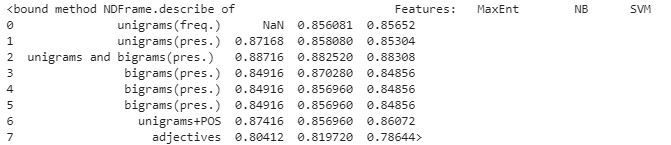
\includegraphics[width=\linewidth]{Base_Article_Results.JPG}
    \end{center}
    
    \item  Figure-2:  Logistic regression
    \begin{center}
         \includegraphics[width=\linewidth]{Logistic_regression_tr.jpg}
    \end{center}
    The figure shows us the top 25 best and worst features. Bar shows us the size of each coefficient using grid best estimator. Negative coefficients on left are indicative of negative reviews. While positive coefficients are indicative of positive reviews.
    
    \item  Figure-3: Scattering of PCA
    \begin{center}
         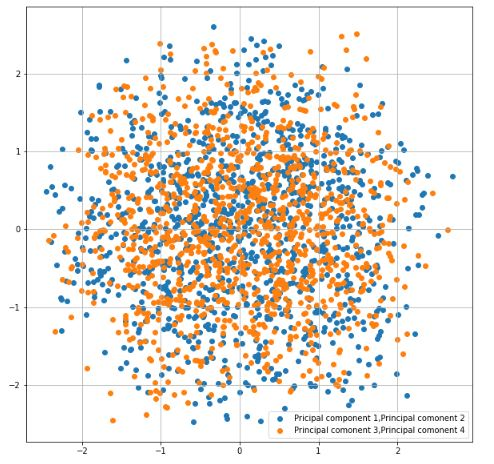
\includegraphics[width=7cm, height=7cm]{Scattering_of_PCA.JPG}
    \end{center}
     This graph shows the scattering of collection of points of 2 columns taken in pair present in dataframe.
    
    \item  Figure-4: Hexbin plot of PCA
    \begin{center}
        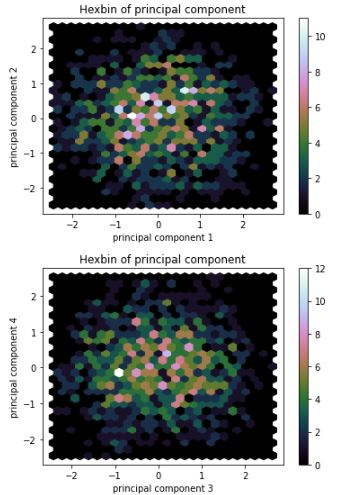
\includegraphics[width=7cm, height=10cm]{Hexbin_of_principal_component.JPG}
    \end{center}
    Hexbin plot represent the relationship of 2 numerical variables when you have a lot of data point. Instead of overlapping, the plotting window is split into several hexbins, and the number of points per hexbin is counted. The colour denotes this number of points.
    
    \item  Figure-5: Cumulative explained variance
     \begin{center}
         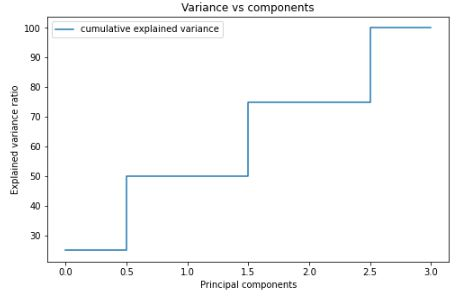
\includegraphics[width=7cm, height=7cm]{Cumulative_explained_variance.JPG}
     \end{center}
     It shows cumulative variance. It is found from individual variance and latter is found from sum of eigenvalues and eigenvalues.
    
    \item  Figure-6: Scattering of Kmeans of PCA
    \begin{center}
         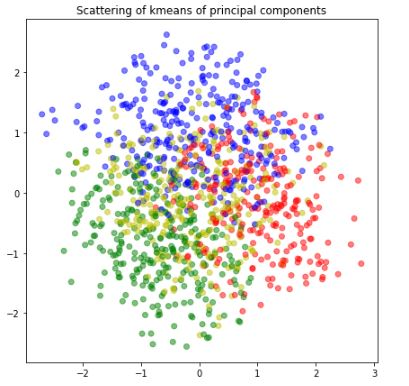
\includegraphics[width=7cm, height=7cm]{Scattering_of_Kmeans_of_PCA.JPG}
    \end{center}
     Shows cluster indices and cluster centre of our PCA data. It also shows the normalized value of all the components.
    
    \item  Figure-7: Pairwise relationship of PCA projected data through KMeans
    \begin{center}
         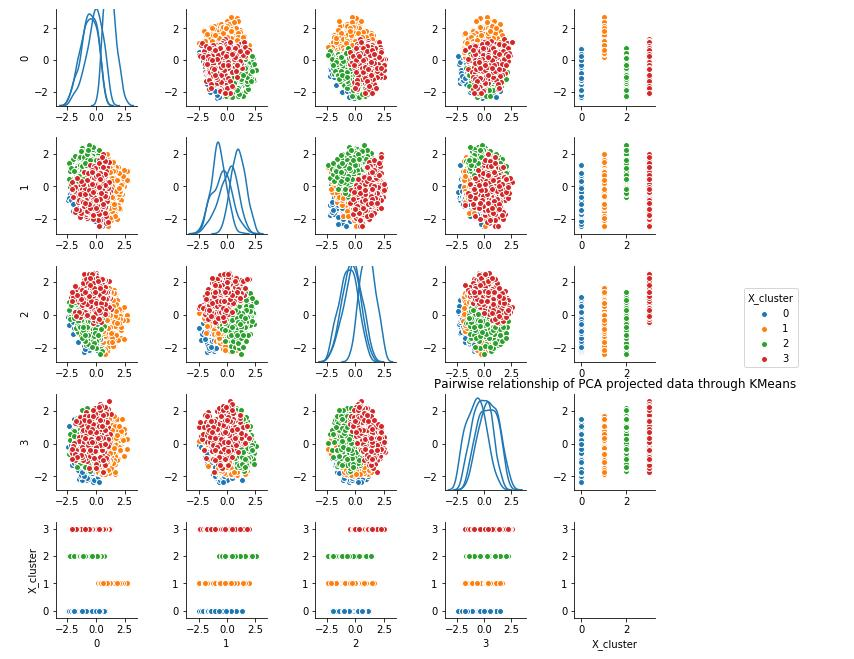
\includegraphics[width=\linewidth]{Pairwise_relationship.jpg}
    \end{center}
     Showing pairwise relationship to visualize our Kmeans clustering on PCA projected data(Seaborn pairplot)
    
    \item  Figure-8: SVM Classifier
    \begin{center}
         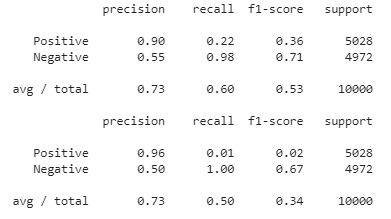
\includegraphics[width=\linewidth, height=5cm]{SVM_Classifier.jpg}
    \end{center}
    The figure shows the classification report of both bag of words(count vectorizer) and tfidf features. In the classification report, it shows precision, support, f1 score, recall of pos and neg.
\end{itemize}

\section{Conclusions}
\begin{itemize}
	\item We can conclude from our base article results that how well different model or classifiers can be applied on the same dataset by calculating accuracy on different features. We also came to know by applying logistic regression on  how to train model, fit model with best  grid estimator, using cross validation to find accuracy score of model and also predict binary output (1 or 0). 
 
    By applying PCA we learnt how to dimensionally reduce the data  from high dimensional data to low dimensional data  to make system faster. We also learnt to calculate  eigenvalue and eigenvector, mean, variance. 

    By applying SVM we learnt how to classify data points or features into positive and negative on basis of polarity 1 and 0 and also on basis of positive and negative tagging. We also learnt to speed up accuracy of system by increasing regularization parameters and  selecting particular classifier, random state.
\end{itemize} 

\newpage
\section{ Contribution of team members}	
\subsection{Technical contribution of all team members }
\begin{table}[h]
\centering
\begin{tabular}{|l|l|l|l|}
    \hline
    Tasks  & Team member 1 & Team member 2 & Team member 3 \\ \hline
    Analysis and Theoretical Support & Aditya & Nilay & \\ \hline
    Pseudo Code & Nilay & & \\ \hline
    Coding and Simulation & Aditya & Dhruvil & Varun \\ \hline
    Errors and Queries & Dhruvil & Varun & \\ \hline
\end{tabular}
\end{table}

\subsection{Non-Technical contribution of all team members }
\begin{table}[h]
\centering
\begin{tabular}{|l|l|l|l|}
    \hline
    Tasks  & Team member 1 & Team member 2 & Team member 3 \\ \hline
    Documentation & Aditya & Varun & \\ \hline
    Integration of modules  & Dhruvil & Nilay & \\ \hline
\end{tabular}
\end{table}

\bibliography{ref.bib}
\bibliographystyle{ieeetr}

\end{document} 